\PassOptionsToPackage{quiet}{fontspec}
\documentclass[UTF8]{ctexart}
\usepackage{titlesec}
\usepackage{fancyhdr}
\usepackage{geometry}
\usepackage{listings}
\usepackage{xcolor}
\usepackage{graphicx}
\usepackage{amsmath}  % 提供了高级数学公式环境
\usepackage{amsfonts} % 提供数学字体
\usepackage{amssymb}  % 提供额外的数学符号

\geometry{left=1.0in,right=1.0in,top=0.3in,bottom=0.3in}

\pagestyle{fancy}
\fancyhf{} % 清空当前的页眉和页脚
\fancyfoot[C]{\thepage} % 页脚中间显示页码

\ctexset{
    section={%
        format=\raggedright\Large\bfseries,
        afterskip=10pt,
    },
    subsection={%
        format=\raggedright\normalsize,
        afterskip=8pt,
    }
}

\lstset{
    language=C++, 
    basicstyle=\ttfamily\small, % 字体样式和大小
    keywordstyle=\color{blue}, % 关键字颜色
    commentstyle=\color{gray}, % 注释颜色
    stringstyle=\color{red}, % 字符串颜色
    numbers=left, % 显示行号
    numberstyle=\tiny\color{gray}, % 行号样式
    frame=single, % 代码框
    breaklines=true, % 自动换行
    captionpos=b % 标题位置
}


\begin{document}

\title{\vspace{0cm}d森林问题实验报告}
\author{程远2234412848}
\date{}
\maketitle
\tableofcontents
\newpage

\section{问题描述}
设T为一带权树,树中的每个边的权都为整数。又设S为T的一个顶点的子集,从T中删除S中的所有结点,
则得到一个森林,记为T/S。如果T/S中所有树从根到叶子节点的路径长度都不超过d,则称T/S是一个d森林。
设计一个算法求T的最小顶点集合S,使T/S为一个d森林。

\section{问题分析}
如果某条路径的长度超过d,则可以通过移除路径中的某些节点将路径拆分为更短的子路径。
如果要使得移走的节点数最少,那应该尽量移走同时在多个长度大于d路径中出现的节点。

贪心思路如下:
1. 通过DFS从叶子计算每个节点到其叶子节点的最大距离,判断该节点是否要移走。
2. 自底向上遍历,使得每次移走节点的收益都最大,即尽可能移走同时在多个长度大于d路径中出现的节点。

\section{算法设计}
算法分为以下几步:
1.通过输入构造树:
由于输入时按照节点编号依次给出节点的子节点与对应的权重,所以不适合使用链式结构储存树。
我通过一个节点向量$vector<\!node\!>\;\;tree$储存每一个节点,其中$tree[0]$为根节点。
2.通过DFS思想算出当前节点到叶子节点的最大距离,需要注意处理节点已经被删除的特殊情况。
3.从叶子节点开始遍历树,依次计算每一个节点到叶子节点的最大距离,与d比较并决定是否删除。
4.统计删除节点个数,输出结果。


\section{算法实现}
以下为具体代码,解释以注释的形式给出
\begin{lstlisting}[language=C++]
int rem[10000]; //用于标记节点是否被移除,rem[i]为1说明i节点已被移除

struct node {
public:
    int index;
    vector<pair<int, int>> children; //children.first为子节点索引,children.second为当前节点与该子节点之间的边的权重
    node(int index_ = -1, const vector<pair<int, int>>& children_ = {})
        : index(index_), children(children_) {}
};

class dTree {
public:
    int n; //节点数
    int d; //最长距离
    vector<node> tree; //记录所以节点的向量

    dTree(int n_ = -1, int d_ = -1) : n(n_), d(d_) 
    {
        for (int i = 0; i < n; i++) 
        {
            vector<pair<int, int>> tempVector;
            int numOfChildren;
            cin >> numOfChildren; 
            if (numOfChildren == 0) 
            {
                tree.emplace_back(i); //用emplace_back()代替push_back()可以节省开销
                continue;
            } 
            else 
            {
                for (int j = 0; j < numOfChildren; j++) 
                {
                    pair<int, int> tempPair;
                    cin >> tempPair.first >> tempPair.second; //依次输入子节点索引和权重
                    tempVector.emplace_back(tempPair);
                }
            }
            tree.emplace_back(i, tempVector);
        }
    }

    int findMaxDistance(int current) //计算当前节点到叶子节点的最大距离
    {
        if (tree[current].children.empty()) //已经为叶子节点,返回0
        {
            return 0;
        }
        int maxDistance = 0;
        for (auto &[child, weight] : tree[current].children) 
        {
            if (rem[child] == 1) continue; //跳过已移除节点
            maxDistance = max(maxDistance, findMaxDistance(child) + weight); //递归调用,找到最大距离
        }
        return maxDistance;
    }

    void solution() //求解最小顶点集合
    {
        int count = 0;
        for (int i = n - 1; i >= 0; i--) //输入按照自上而下顺序,逆序即可实现从子节点开始遍历
        {
            int maxDistance = findMaxDistance(i);
            if (maxDistance > d) 
            {
                rem[i] = 1; // 移除该节点
                count++;
            }
        }
        cout << count << endl;
    }
};

\end{lstlisting}

\section{运行结果}
通过moodle上所有用例
\begin{figure}[htbp]
    \centering
    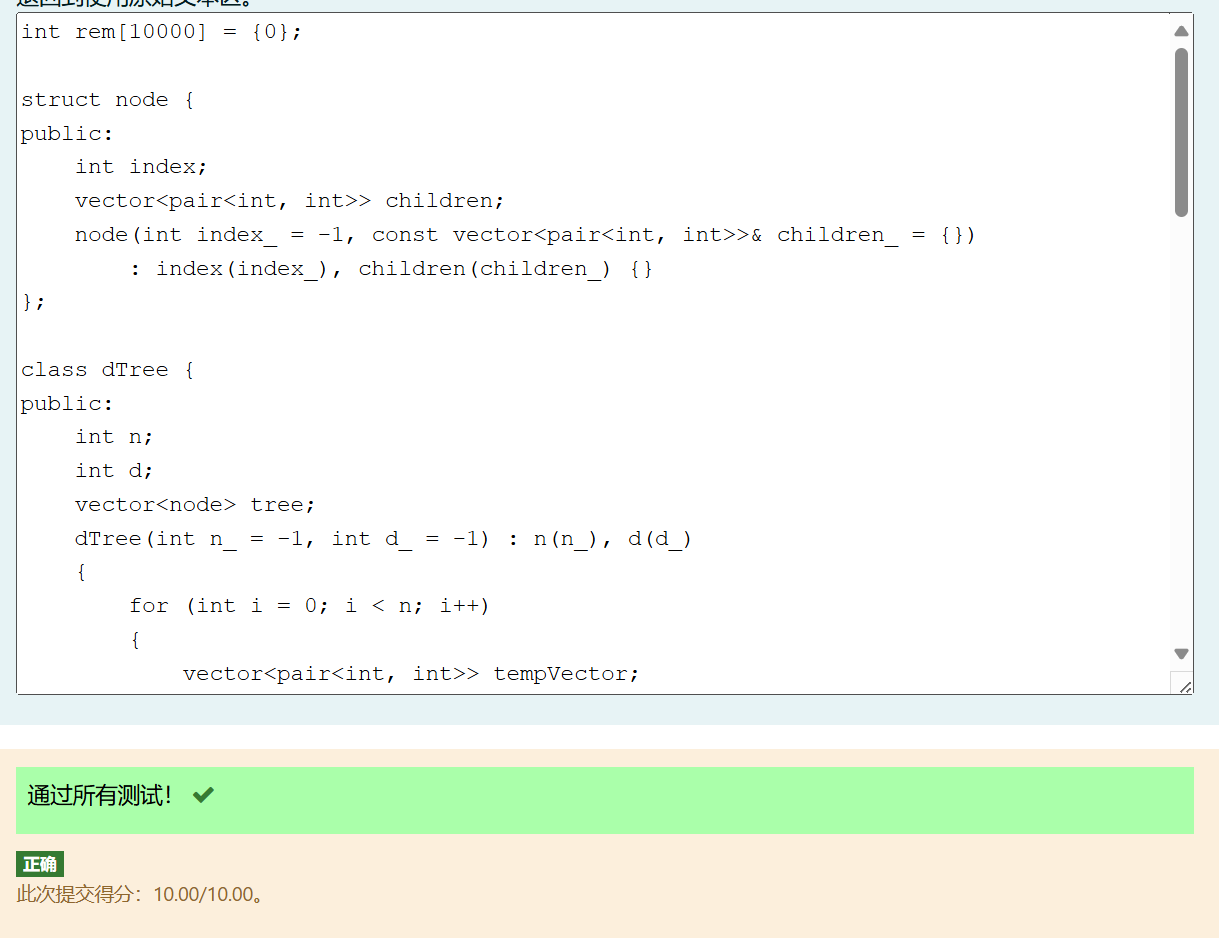
\includegraphics[width=0.8\textwidth]{moodle1.png}
\end{figure}

\section{复杂度分析}
1. 时间复杂度:
    构建树时的复杂度为 $O(n)$。
    遍历所有节点需要$n$次
    每个节点的 DFS 计算复杂度为 $O(n)$。
    总复杂度为 $O(n^2+n) = O(n^2)$。


2. 空间复杂度:
    存储树结构需要 $O(n)$ 的空间。
    额外的标记数组 'rem'占用 $O(n)$ 的空间。
    总空间复杂度为 $O(n)$。

\section{算法优化}
通过动态规划,使用maxDist动态记录已经计算出最大距离节点的距离,再次遇到该节点时便可省去计算。
最终相当于只进行了一次findMaxDistance操作,递归函数时间复杂度由$O(n^2)$降至$O(n)$。总复杂度也降为$O(n)$具体优化代码如下,仅需修改findMaxDistance函数:
\begin{lstlisting}[language=C++]
    int maxDist[10000]; //添加记录数组,记录对应节点的最大距离
    int findMaxDistance(int current) 
    {
        if(tree[current].children.empty()) 
        {
            return 0;
        }
        if(maxDist[current] != 0) return maxDist[current]; //已经计算过的节点,直接调用结果
        int maxDistance = 0;
        for(auto &[child, weight] : tree[current].children) 
        {
            if(rem[child] == 1) continue;
            maxDistance = max(maxDistance, findMaxDistance(child) + weight);
        }
        maxDist[current] = maxDistance; //记录已经计算过的节点的最大距离
        return maxDistance;
    }

\end{lstlisting}

\section{浅浅反思}
编程过程中花了大量时间构造树与写dfs,说明数据结构还是不够熟练:(。
\end{document}
